\documentclass[12pt,a4paper]{article}
\usepackage[utf8]{inputenc}
\usepackage{amsmath}
\usepackage{amsfonts}
\usepackage{amssymb}
\usepackage{graphicx}
\usepackage{subcaption}
\usepackage{float}

\author{Team Gamma}
\title{Observation model}
\date{}
\begin{document}
	
	\maketitle
	
	When evaluating our model performance, we focused on two things - face detection speed and number of frames where our face was detected. We have tested three different face detectors, two from dlib library and one from opencv.
	
	\section{Speed}
	
	All the tests were done on realtime video that was streaming to the topic \texttt{camera/raw\_image} (similar to the turtlebot configuration that we will be using for our final task). We could process each frame individually, but that would defeat the purpose of our face detector. We wanted to make sure, that it can be run realtime on our robot and produce good results. \\
	
	In the opencv implementation, we are using haar cascade, which was and is widely used in cameras as it is very fast and can be run in realtime. \\
	
	We have also tested dlib's HOG and CNN detector. The HOG detector is extremly fast, the fastest of the three. We have, on the other hand, observed, that the dlib's convolutional neural network face detection is slow and cannot be run in realtime. \\
	
	In the table below, we compare the processing speed of different detectors. We are interested in how many frames the algorithm can process, and the number of frames that the face was detected in. If the resolution of the image is too low, the faces will most likely not be detected at all. \\
	
	\begin{center}
		\begin{tabular}{|c|c|c|c|}
			\hline 
			Detector & Frame size & Processed frames & Face detections \\ 
			\hline
			dlib HOG & 1920 x 1080 & 22 / 130 & 9 \\
			dlib HOG & 960 x 540 & 69 / 130 & 18 \\
			dlib HOG & 480 x 270 & 130 / 130 & 18 \\
			dlib CNN & 1920 x 1080 & 1 / 130 & 0 \\
			dlib CNN & 960 x 540 & 1 / 130 & 0 \\
			dlib CNN & 480 x 270 & 4 / 130 & 0 \\
			opencv haar cascade & 1920 x 1080 & 8 / 130 & 8 \\
			opencv haar cascade & 960 x 540 & 26 / 130 & 18 \\
			opencv haar cascade & 480 x 270 & 90 / 130 & 29 \\
			\hline 
		\end{tabular} \\
	\end{center}
	
	As we can see, the dlib HOG detector is the fastest - it can process frames in real time. The dlib CNN detector is the slowest - it can only process one frame before the video ends. This shows that the CNN detector can not be used to detect faces in our finished product. \\
	
	The opencv is not quite as fast as the dlib HOG detector, but it can process data almost in realtime and it actually detects the face very well - even better than HOG. \\
	
	The Kinect video resolution is \texttt{640 x 480}, which means that we will be able to process it using either HOG or haar cascade detector. For that reason the following tests were performed on HOG and haar cascade detectors only. \\
	
	\section{Face detection}
	
	For face detection we did not know whether it is better to use black and white image or color one, so we tested each of the two options. We found out that detectors performed better with monochromatic images. \\
	
	We also wanted to find the best image resolution at which the number of correctly recognized faces is the largest, so we tested three different resolutions: \texttt{960 x 540}, \texttt{480 x 270} and \texttt{240 x 135}. Both detectors were able to detect faces in almost real time, but we found out that the resolution at which most faces were recognized correctly was the \texttt{960 x 540}. That means that for the best performance in the final task, we will use the largest image that Kinect sensor can produce, that is \texttt{640 x 480}. \\
	
	In the table below we can see the number of true positives (TP), false positives (FP) and false negatives (FN) for each detector. 
	True positives are correctly detected faces, false positives incorrectly detected faces, and false negatives represent the number of processed frames with no detected faces.
	We can see that the HOG detector has way more false negatives than the Haar detector, which shows two things. First, Haar detector is better at detecting faces (considering the number of processed frames) and secondly, HOG detector is much faster and it can process more frames than Haar detector.
	
	
	\begin{center}
		\begin{tabular}{|c|c|c|c|c|c|c|}
			\hline 
			& \multicolumn{3}{c|}{HOG detector score} & \multicolumn{3}{c|}{Haar detector score} \\
			\hline
			Video & TP & FP & FN & TP & FP & FN \\
			\hline 
			\texttt{ face01\_0deg } & 75 & 0 & 163 & 56 & 15 & 35 \\
			\texttt{ face01\_30deg } & 58 & 0 & 138 & 47 & 2 & 30 \\
			\texttt{ face01\_45deg } & 0 & 0 & 1 & 52 & 2 & 44 \\
			\texttt{ face01\_60deg } & 58 & 0 & 167 & 18 & 2 & 70 \\
			\texttt{ face02\_0deg } & 20 & 0 & 60 & 17 & 0 & 11 \\
			\texttt{ face02\_30deg } & 33 & 0 & 81 & 24 & 0 & 16 \\
			\texttt{ face02\_45deg } & 25 & 0 & 78 & 15 & 0 & 25 \\
			\texttt{ face02\_60deg } & 10 & 0 & 104 & 8 & 0 & 36 \\			
			\hline 
		\end{tabular} \\
	\end{center}
	
	In the table below we can see the comparison between haar cascade and HOG face detector performance on different files. We used videos of 2 different faces taken at 4 different angles each. The file resolution is 960 x 540. The score is calculated as $\frac{\text{number of true positives}}{\text{number of frames}}$.
	
	\begin{center}
			\begin{tabular}{|c|c|c|}
			\hline 
			Video & HOG detector score & Haar detector score \\
			\hline
			\texttt{face01\_0deg} & 0.32 & 0.62 \\
			\texttt{face01\_30deg} & 0.3 & 0.61 \\
			\texttt{face01\_45deg} & 0.0 & 0.54 \\
			\texttt{face01\_60deg} & 0.26 & 0.2 \\
			\texttt{face02\_0deg} & 0.25 & 0.61 \\
			\texttt{face02\_30deg} & 0.29 & 0.6 \\
			\texttt{face02\_45deg} & 0.24 & 0.38 \\
			\texttt{face02\_60deg} & 0.09 & 0.18 \\
			\hline 
		\end{tabular} \\
	\end{center}


	As we can see, the \textbf{opencv haar cascade detector} performed better than the other. It correctly identified twice as much faces in all videos. \\

	\section{Face detector performance}
	
	Now that we have selected our face detector, we can use it to estimate its performance for any distance and angle to the face. The results are plotted in the following graph. \\
	
	On x axis we have distance to the face in intervals of 0.5m, on y axis we can see the ngles from which the face was approached, and on the z axis we have the number of correctly detected faces (true positives) for each distance-angle pair. \\
	
	\begin{center}
		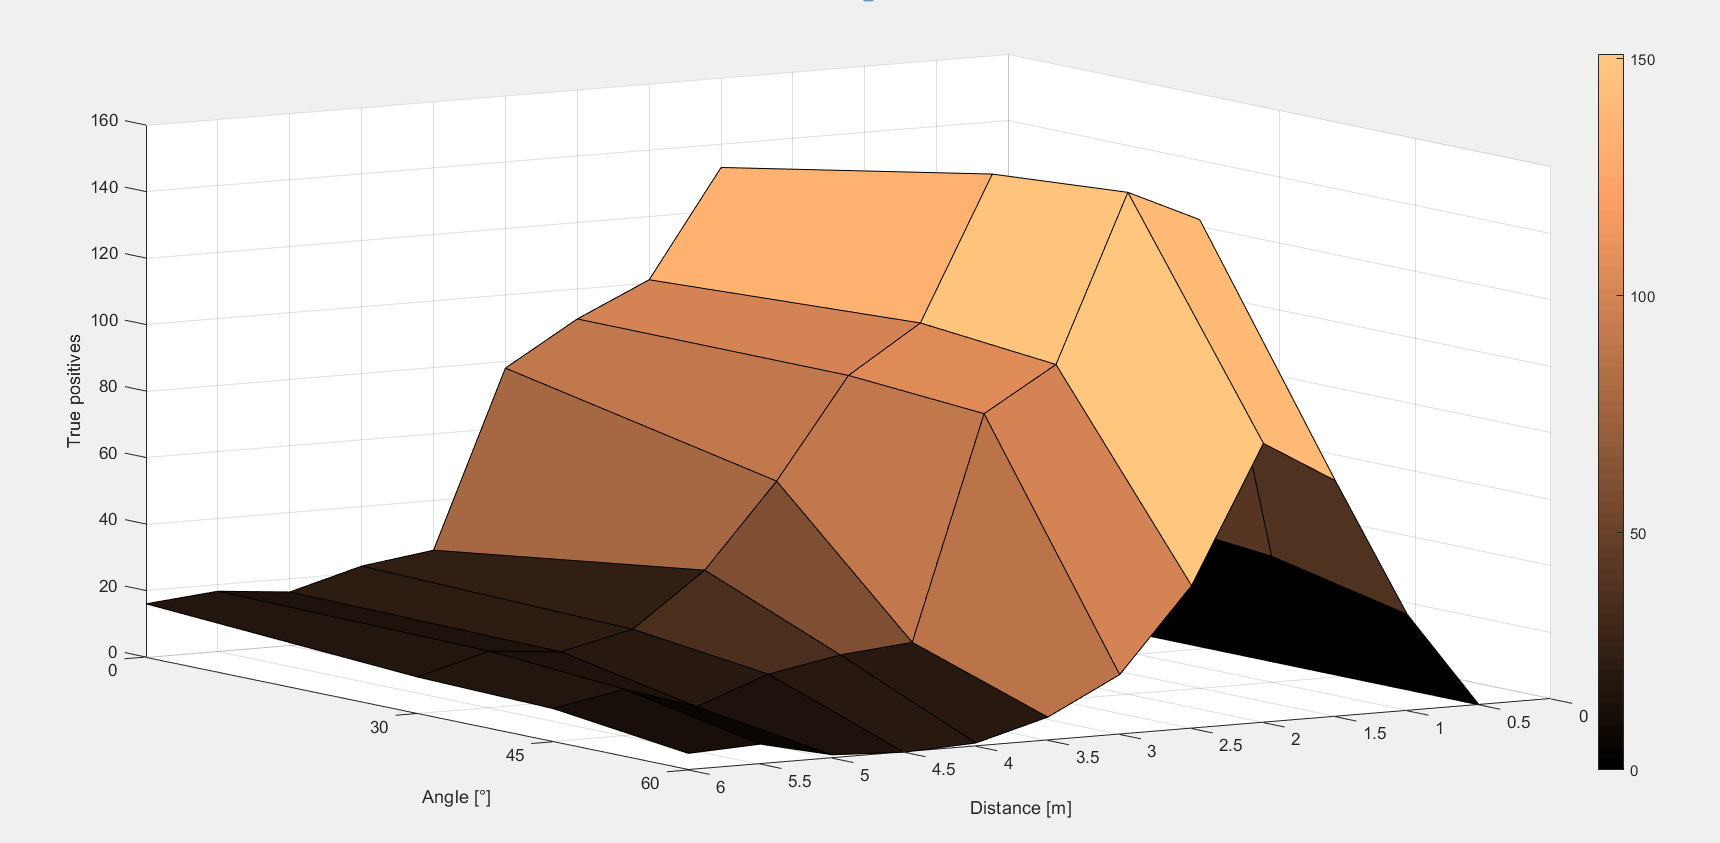
\includegraphics[width=.6\linewidth]{graf4}
	\end{center}
	
	\begin{figure}[H]
		\begin{subfigure}{.5\linewidth}
			\centering
			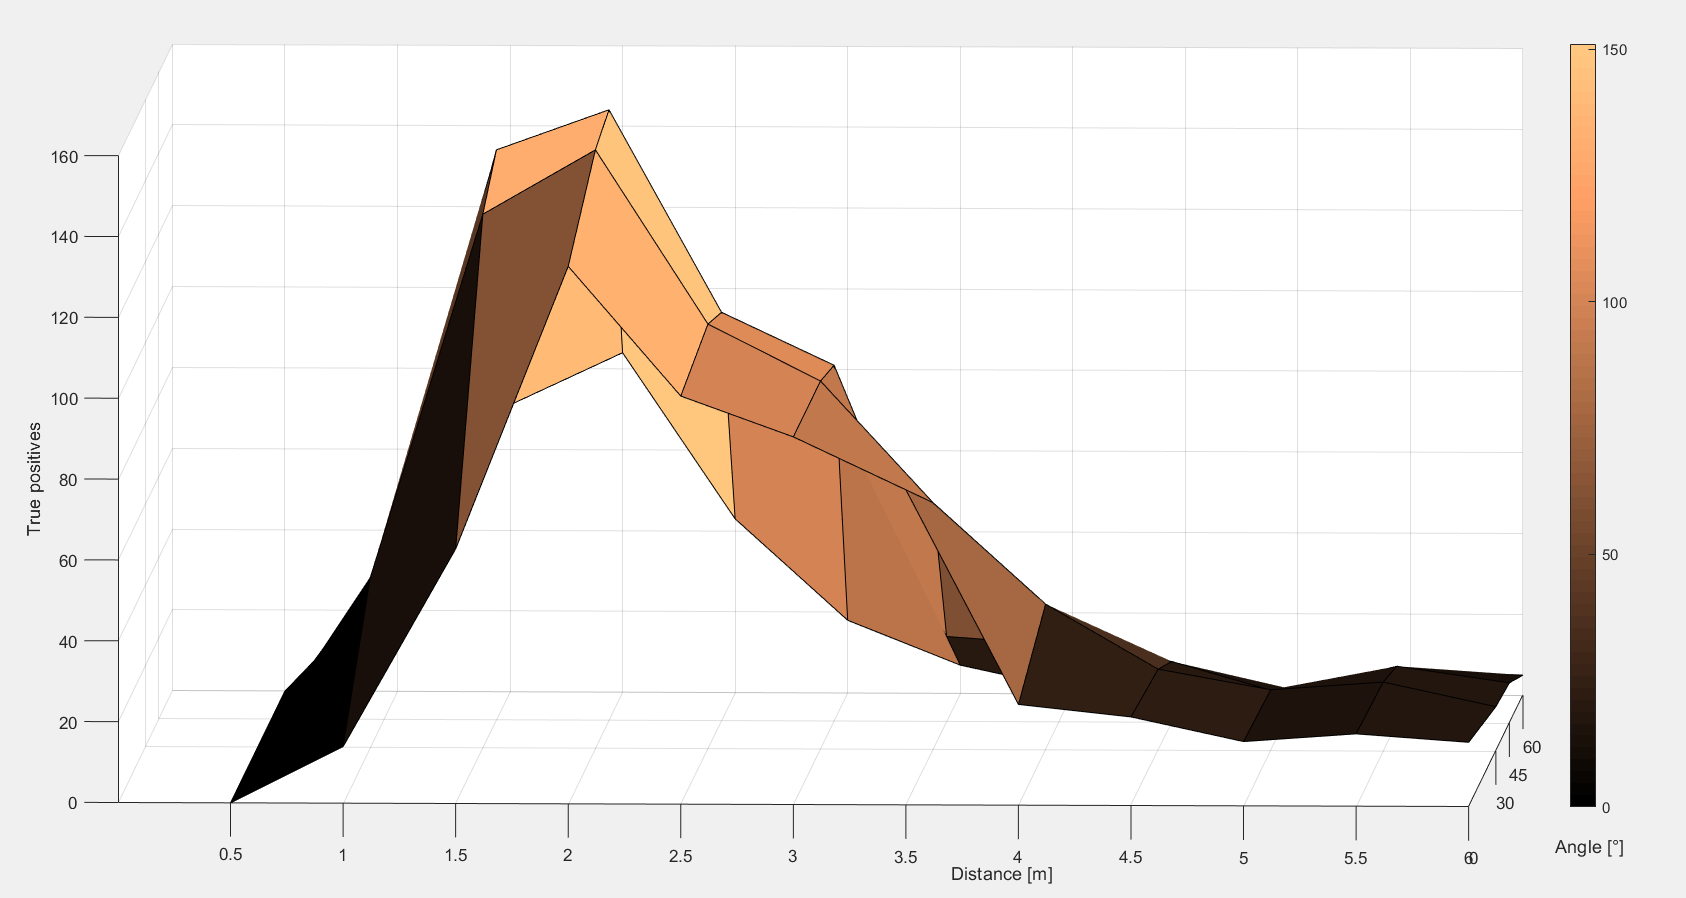
\includegraphics[width=.8\linewidth]{graf5}
		\end{subfigure}
		\begin{subfigure}{.5\linewidth}
			\centering
			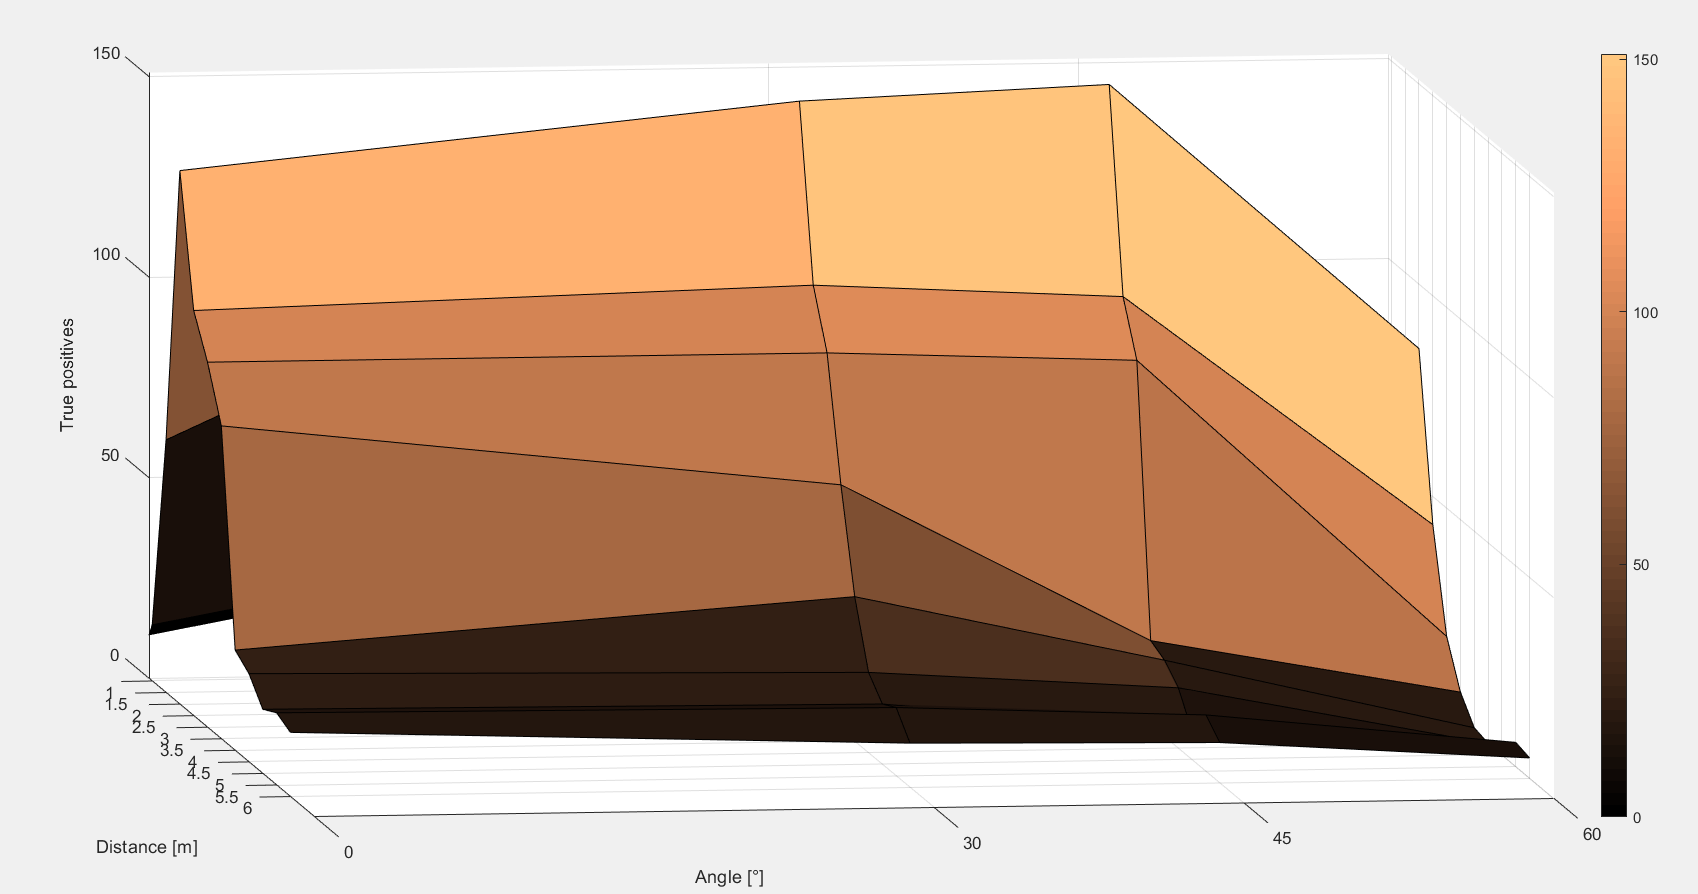
\includegraphics[width=.8\linewidth]{graf6}
		\end{subfigure}
	\end{figure}

	We can see that detection works best at the distance of 1.5 and 2.5 meters. The diference between different angles aren't as noticable. The detector works a bit worse when video is taken from a large, 60$^{\circ}$ angle. \\
	
	In conclusion, our test showed that the best way to detect faces with our robot is the following:
	\begin{enumerate}
		\item Convert rgb images to grayscale before running the detector
		\item Use opencv haar cascade detector for face detection
		\item Use the biggest resolution of the images that kinect can provide
		\item If possible, try to perform face detection at the distance between 1.5 and 2.5 meters from the possible face locations
		\item Make sure that the angle at which you approach possible face location isn't too big
	\end{enumerate}	
	
\end{document}